\documentclass[aspectratio=169]{beamer}
\beamertemplatenavigationsymbolsempty
\usepackage{qrcode}

\usepackage{parskip, setspace}
\setstretch{1.5}

% \usepackage{biblatex}
% \addbibresource{bib.bib}
% math formatting
\usepackage{amsmath, amsfonts, braket}
% \numberwithin{equation}{section}
% rich text
\usepackage{graphicx, caption}
\usepackage{hyperref}
\usepackage{xcolor}
\hypersetup{
    colorlinks=false,
    linkcolor=black,  
    urlcolor=blue,
    citecolor=blue,
    pdftitle={Chapman APS NW 2024},
    pdfpagemode=FullScreen,
}

\usepackage[ruled,linesnumbered,lined,boxed,commentsnumbered]{algorithm2e}

\usetheme{Madrid}
\title[Analog Particles with HPC]{Modelling Particle Production in Analog Expanding Universes with High-Performance Computing}
% \subtitle{}

\author[Chapman, Nathaniel]{Nathaniel Chapman}

\institute[CWU]
{
  Department of Computer Science \\
  Department of Physics \\
  Central Washington University
%   \and
%   \inst{2}%
%   Faculty of Chemistry\\
%   Very Famous University
}

\date[APS NW 2024]{APS NW 2024}

\logo{
\includegraphics[height=0.5cm]{images/cwu_logo.png}}

\begin{document}

\frame{\titlepage}

\section{Introduction}
\subsection{}
\begin{frame}
    \frametitle{Introduction - Analog Universes}

    \begin{columns}
        \begin{column}{0.5\textwidth}
            \begin{enumerate}
                \item <1->Inflation created particles
                \item <2->Cannot directly observe these particles
                \item <3->Theory suggests ultra-cold quantum gases behave similarily
                \item <4->Can make gas in the lab $\implies$ can \emph{effectively} observe inflation particles
                \item <5->Lab based system = ``analog universe''
            \end{enumerate}
        \end{column}
        \begin{column}{0.5\textwidth}
            \begin{figure}
                \centering
                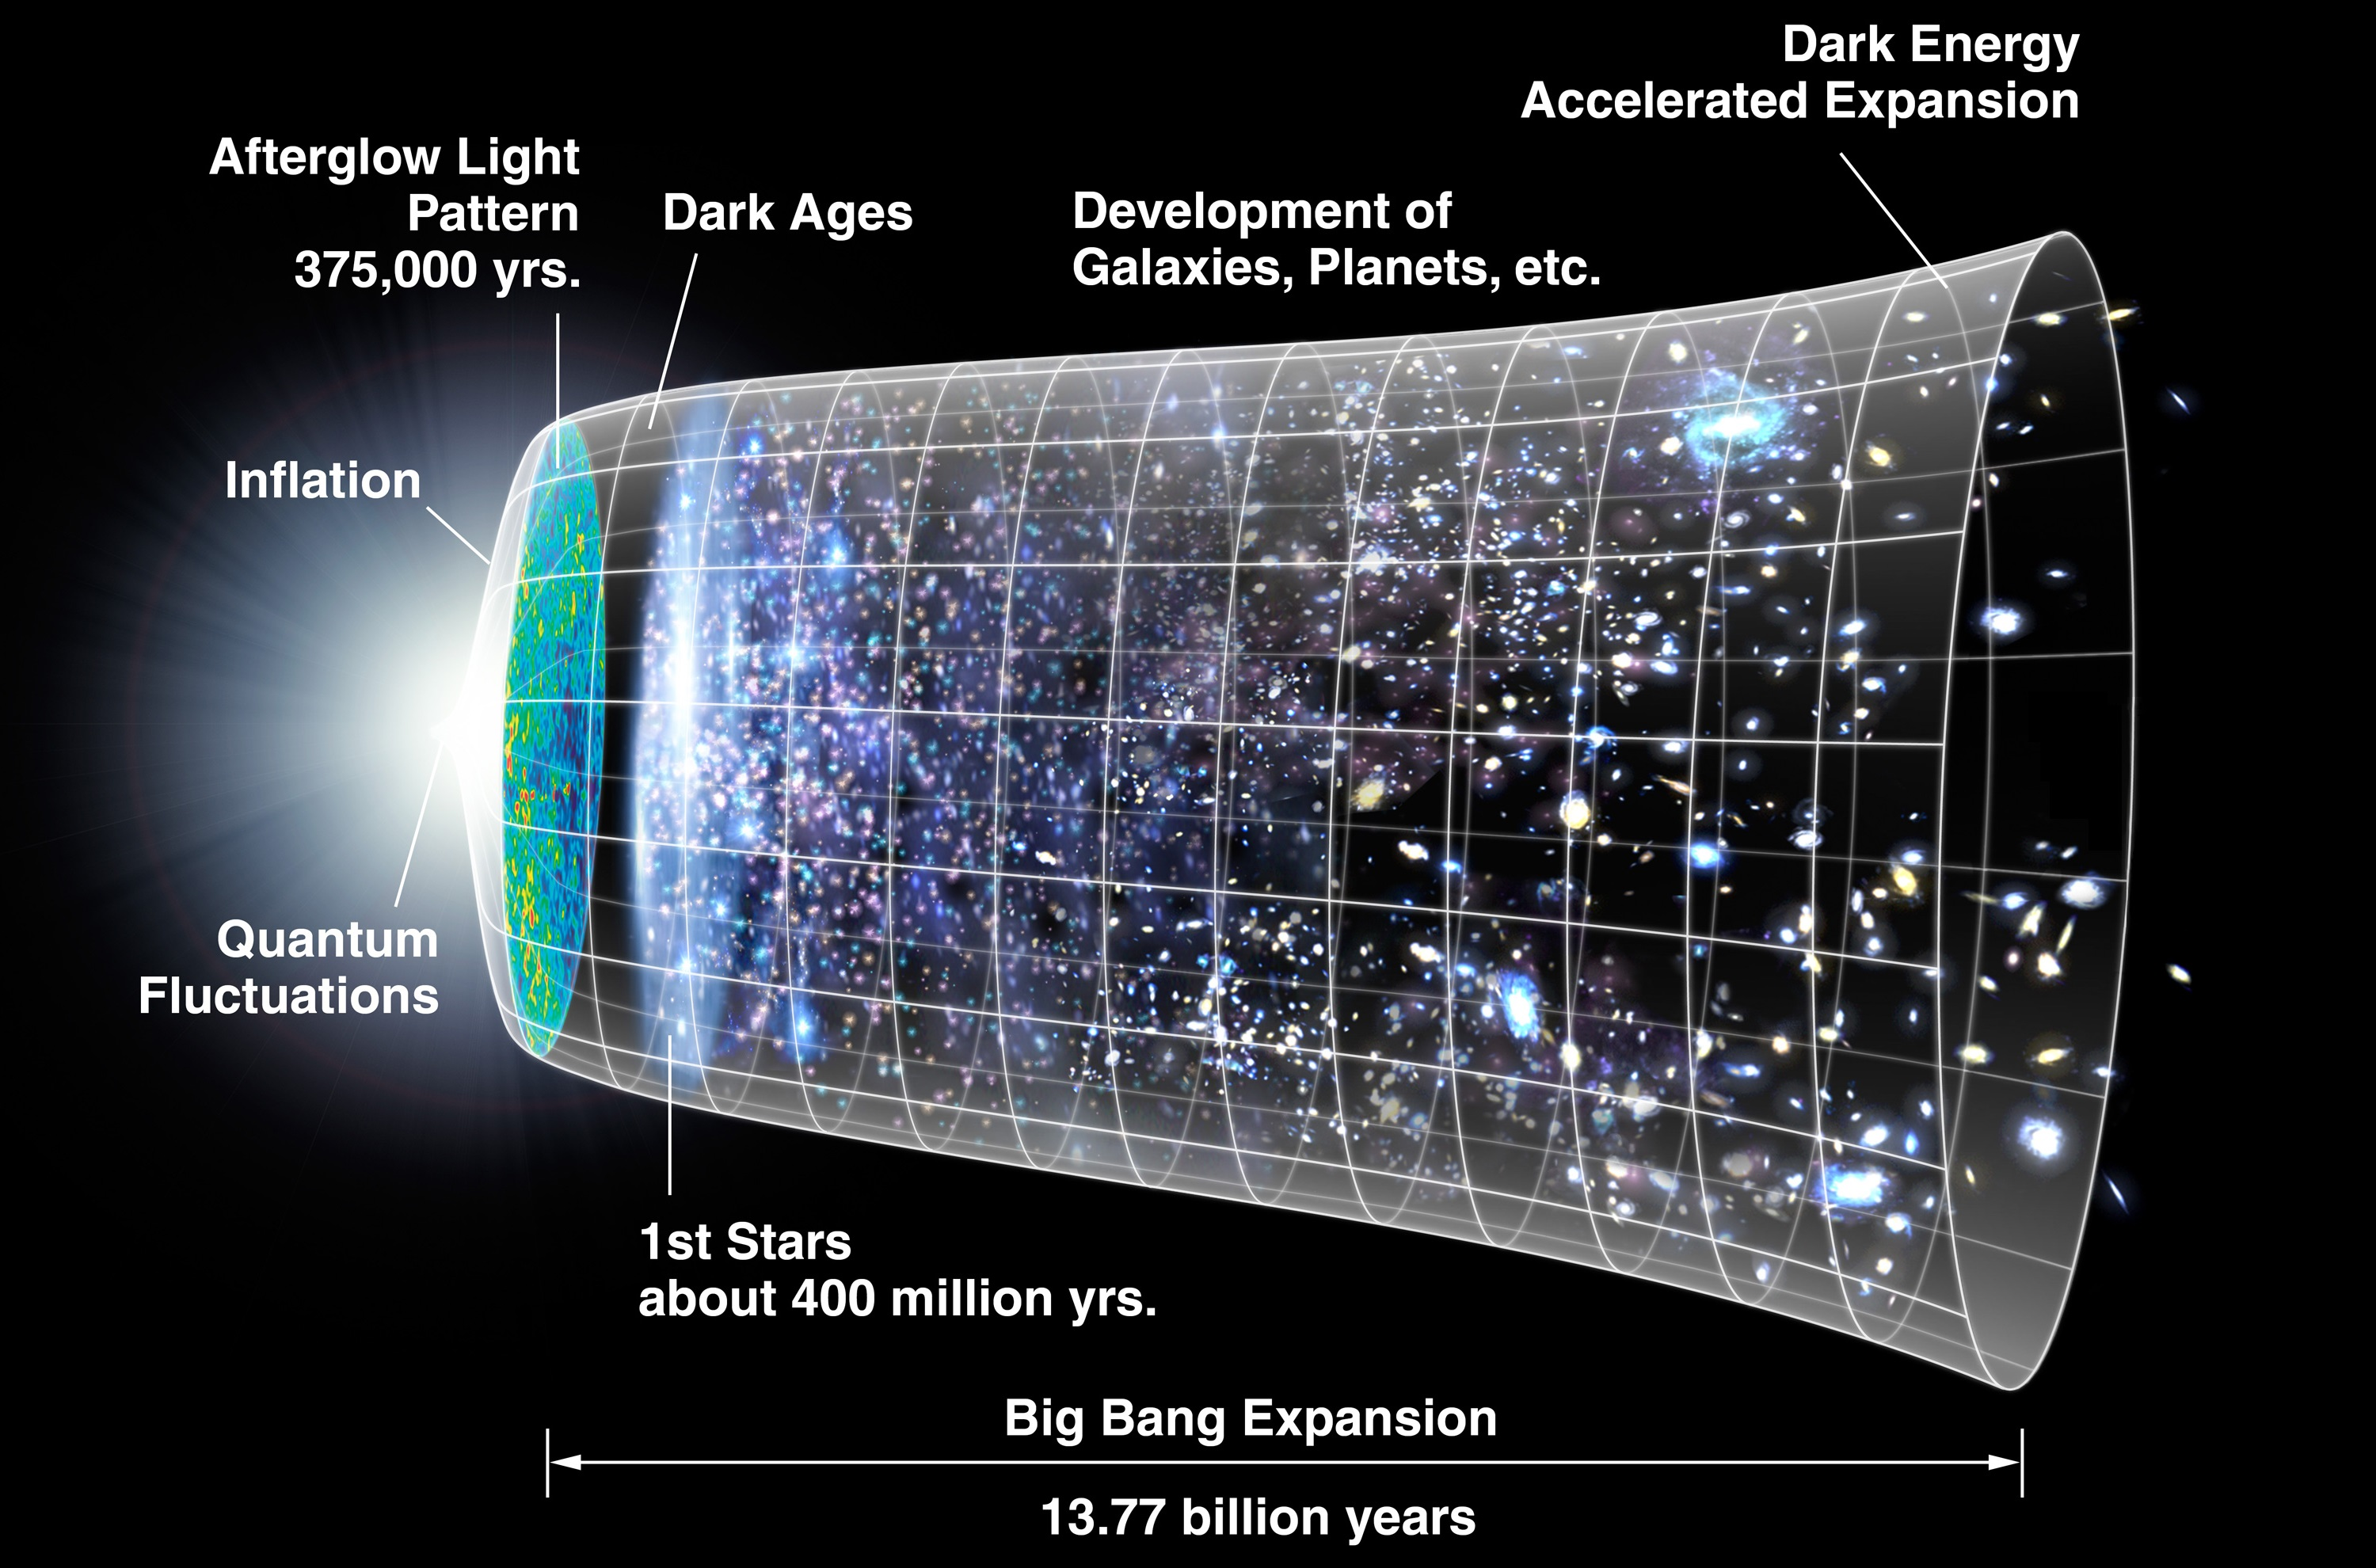
\includegraphics[width=\textwidth]{images/CMB_Timeline300_no_WMAP.jpg}
                \caption{History of the universe highlighting period of rapid expansion (\href{https://upload.wikimedia.org/wikipedia/commons/6/6f/CMB_Timeline300_no_WMAP.jpg}{Source})}
            \end{figure}
        \end{column}
    \end{columns}
\end{frame}

\begin{frame}
    \frametitle{Introduction - The Story So Far}

    \begin{columns}
        \begin{column}{0.5\textwidth}
            \begin{itemize}
                \item <1->Many investigations into analog universes
                \item <2->Few into exact analogs
                \item <3->Fewer into computational simulation
                \item <4->Even fewer using high-performance computing
            \end{itemize}
        \end{column}
        \begin{column}{0.5\textwidth}
            \begin{figure}
                \centering
                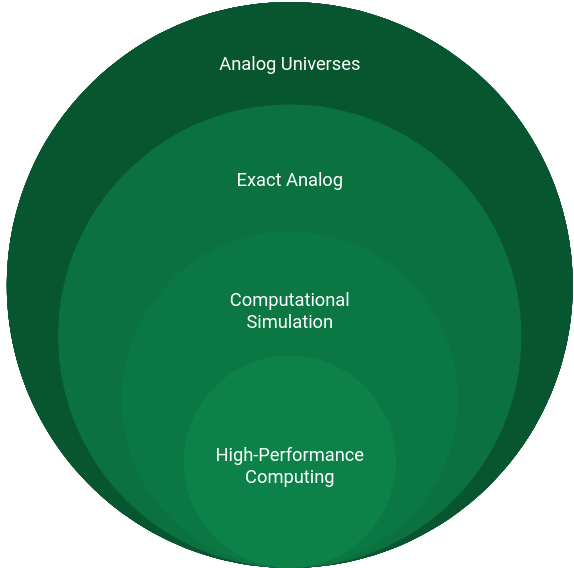
\includegraphics[width=0.7\textwidth]{images/subsets.png}
                \caption{Subsets of increasingly specific literature}
            \end{figure}
        \end{column}
    \end{columns}
\end{frame}
\end{document}